\chapter{Data Acquisition and Processing}
\label{ch:Data Acquisition and Processing}

\section{CUORE Data Acquisition}
Because of the need in CUORE to calibrate $\sim$monthly, there are multiple layers for how data is organized for CUORE.
At the largest scales, there are datasets that begin and end during these monthly calibrations where the closing calibration for one dataset can be used as the opening calibration for the following dataset.
Composing each dataset are runs of $\sim24$ hour length.
These runs are further broken down into 3 types: `background' for physics runs, `calibration' for calibration runs, and `test' runs.
The test runs can be much more varied than the 24 hour background and calibration runs, and can include runs for various reasons, such as setting the working points of the NTDs or for scanning pulse tube phases.

The towers are numbered according to bla bla in \autoref{fig:CalibrationSources_DAQ}


\begin{figure}
    \centering
    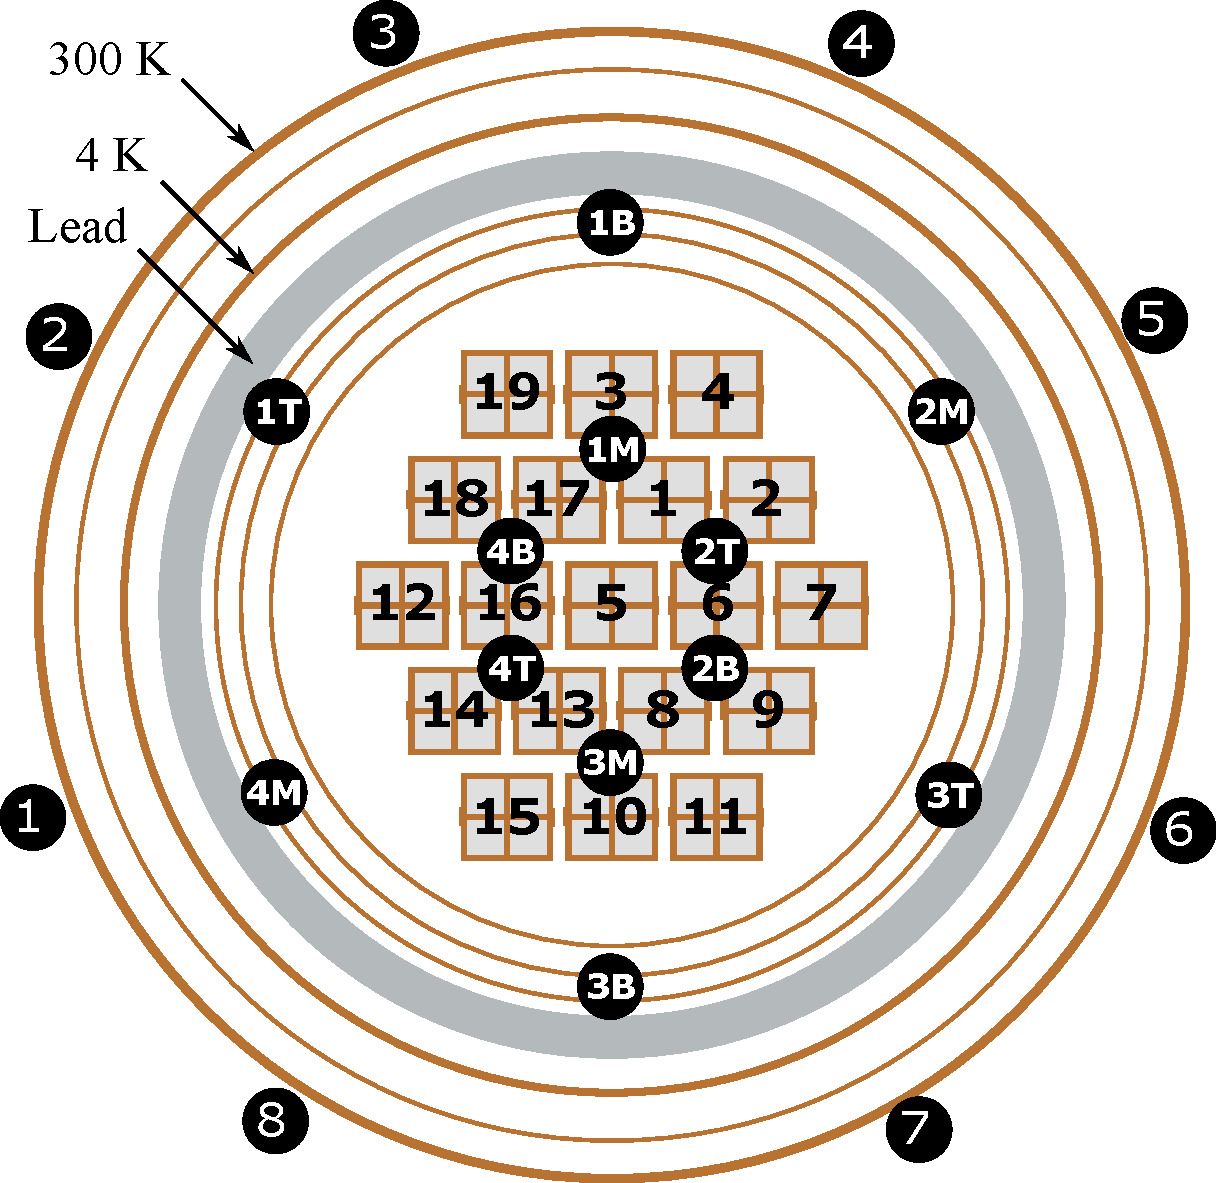
\includegraphics[width= 4 in, height = 4 in, keepaspectratio]{Figures/CalibrationSources_DAQ.pdf}
    \caption[The detector and calibration source numbering for both the inner and outer DCS.]
    {The detector and calibration source numbering for both the inner and outer DCS.}
    \label{fig:CalibrationSources_DAQ}
\end{figure}


\subsection{DAQ Electronics Hardware}
The DAQ is used to read out the data from the componenets
\section{Online Data Taking}
We take data online?
\subsection{Signal Triggering}
We need to trigger on pulses
\section{Offline Data Processing}
We take this data and calculate stuffs
\subsection{First-Level Processing}
\subsubsection{Preprocess}
We prepare stuff for real processing
\subsubsection{Amplitude Evaluation}
We calculate the height of the peaks
\subsubsection{Stabilization}
Need to stabilize at different baselines
\label{ssec:Stabilization}

The energy dissipated in the silicon heater transfers into the bolometer similarly how a real energy deposition would look in a physics event, and allows for us to understand the response of the detector to fixed-energy input across various detector baselines as the temperature of the detectors drifts \cite{ALESSANDRELLO1998454:Si-heater}.

\subsubsection{Calibration}
How do we tell that different calibration rates are correct?
\label{ssec:Calibration}
\subsection{Second-Level Processing}
\subsubsection{Pulse Shape Analysis}
\subsubsection{Coincidence Analysis}



